\documentclass[11pt, a4paper]{article}
\usepackage{graphicx}
\usepackage{amsmath}
\usepackage{listings}
\usepackage{mathrsfs}



\title{Assignment 6} % Title

\author{Om Shri Prasath (EE17B113)} % Author name

\date{\today} % Date for the report
\begin{document}	

\maketitle % Insert the title, author and date
\section{Introduction}\label{introduction}

\begin{itemize}
\item
  We analyse the LTI systems in continuous time using Laplace
  transform to find the solutions to the equations governing the system
  with the help of python tools such as Signal toolbox\\
\item
  \(system.impulse \to\) Computes the impulse response of the transfer
  function
\item
  \(sp.lsim \to\) This simulates \(y=u(t)*h(t)\) taking \(u(t)\) and  $\mathcal{H}(s)$ as arguments
\item
  \(sp.lti \to\) defines a transfer function from polynomial
  coefficients of numerator and denominator as inputs.
\item
  \ $bode() \to $ It's used to find the magnitude and phase response of
  transfer function
\item
  We use following method to find the Laplace transform of a time domain
  signal, here we use these methods to find laplace of system governing
  differential coefficients
\item
  Some of the equations to follow while finding laplace transform
\end{itemize}

\begin{equation}
    \mathscr{L}\{x(t)\} \to \mathcal{X}(s)
\end{equation}

\begin{equation}
    \mathscr{L}\{\frac{dx(t)}{dt}\} \to s\mathcal{X}(s)-x(0^{-})
\end{equation}

\begin{equation}
    \mathscr{L}\{\frac{d^{2}x(t)}{dt^{2}}\} \to s^{2}\mathcal{X}(s)-sx(0^{-})-\dot x(0^{-})
\end{equation}

\begin{itemize}
\item
  Combining the above equations above, we find the laplace transform of
  a differential equation and analyse them.
\end{itemize}
\section{Python Code}\label{code}

\subsection{Question 1 \& 2:}\label{question-1-2}

\begin{itemize}

\item
  To solve for the time repsonse of the spring mass system,whose driving
  force varies as \(f(t)\) given as
\end{itemize}

\begin{equation}
f(t) = \cos(1.5t) e^{-0.5t}u_0(t)
\end{equation}

\begin{itemize}

\item
  Laplace transform of \(f(t)\) using equations (1),(2) \& (3) given
  above
\end{itemize}

\begin{equation}
    \mathcal{F}(s) = \frac{s+0.5}{(s+0.5)^2 + 2.25}
\end{equation}

\begin{itemize}

\item
  Spring satisfies the below equation with \(x(0)\) \(=\) \(0\) and
  \ $\dot x(0) = 0$ for  $ 0 \leq t \leq 50s $.
\end{itemize}

\begin{equation}
\ddot x + 2.25x = f(t)
\end{equation}

\begin{itemize}
\item
  So we take laplace transform of the equation given above with given
  intial conditions and in generalised form considering
  $w_{0}^{2} = 2.25 $ in the differential equation above,
  natural frequency of the system is \(w_0 = 1.5 rads^{-1}\),and decay
  factor of \(f(t)\) as \(d = 0.5\) and frequency of the input as
  $\omega = 1.5 rads^{-1}$ in this question.
\item
  In general we get
\end{itemize}

\begin{equation}
    \mathcal{X}(s) = \frac{s+d}{((s+d)^2 + w^2)(s^2 + w_{0}^{2})}
\end{equation}

\begin{itemize}

\item
  In question 1 we get with given values and \(d = 0.5\)
\end{itemize}

\begin{equation}
    \mathcal{X}(s) = \frac{s+0.5}{((s+0.5)^2 + 2.25)(s^2 + 2.25)}
\end{equation}

\begin{itemize}

\item
  Solve the above problem with much smaller decay with same initial
  conditions, now \(f(t)\) is as follows
\end{itemize}

\begin{equation}
f(t) = \cos(1.5t) e^{-0.05t}u_0(t)
\end{equation}

\begin{itemize}

\item
  So in question 2 we get with \(d = 0.05\)
\end{itemize}

\begin{equation}
    \mathcal{X}(s) = \frac{s+0.05}{((s+0.05)^2 + 2.25)(s^2 + 2.25)}
\end{equation}

\begin{itemize}

\item
  To solve for \(x(t)\) displacement for each of the cases using Laplace
  transform with python tools such as \(system.impulse\) and plot them.
\item
  To analyse the plots obtained and discuss the effect of decay on
  \(x(t)\).
\end{itemize}
\textit{\textbf{Code:}}
   \begin{lstlisting}
def laplaceSolver(decay, w):
    Xn = poly1d([1, decay])
    Xd = polymul([1, 0, pow(w, 2)], [
                 1, 2*decay, (pow(w, 2)+pow(decay, 2))])
    Xs = sp.lti(Xn, Xd)
    t, x = sp.impulse(Xs, None, linspace(0, 100, 10000))
    return Xs, t, x

X, t1, x1 = laplaceSolver(0.5, 1.5)

X, t2, x2 = laplaceSolver(0.05, 1.5)

plot(t1, x1, label="decay = 0.5")
legend()
title(r"Figure 1a: $x(t)$ of spring system")
ylim((-1, 1))
xlabel(r"$t \to $")
ylabel(r"$x(t) \to $")
grid()
show()

plot(t2, x2, label="decay = 0.05")
legend()
ylim((-8, 8))
title(r"Figure 1b: $x(t)$ of spring system")
xlabel(r"$t \to $")
ylabel(r"$x(t) \to $")
grid()
show()
   \end{lstlisting}
\newpage
\begin{figure}[!tbh]
    \centering
    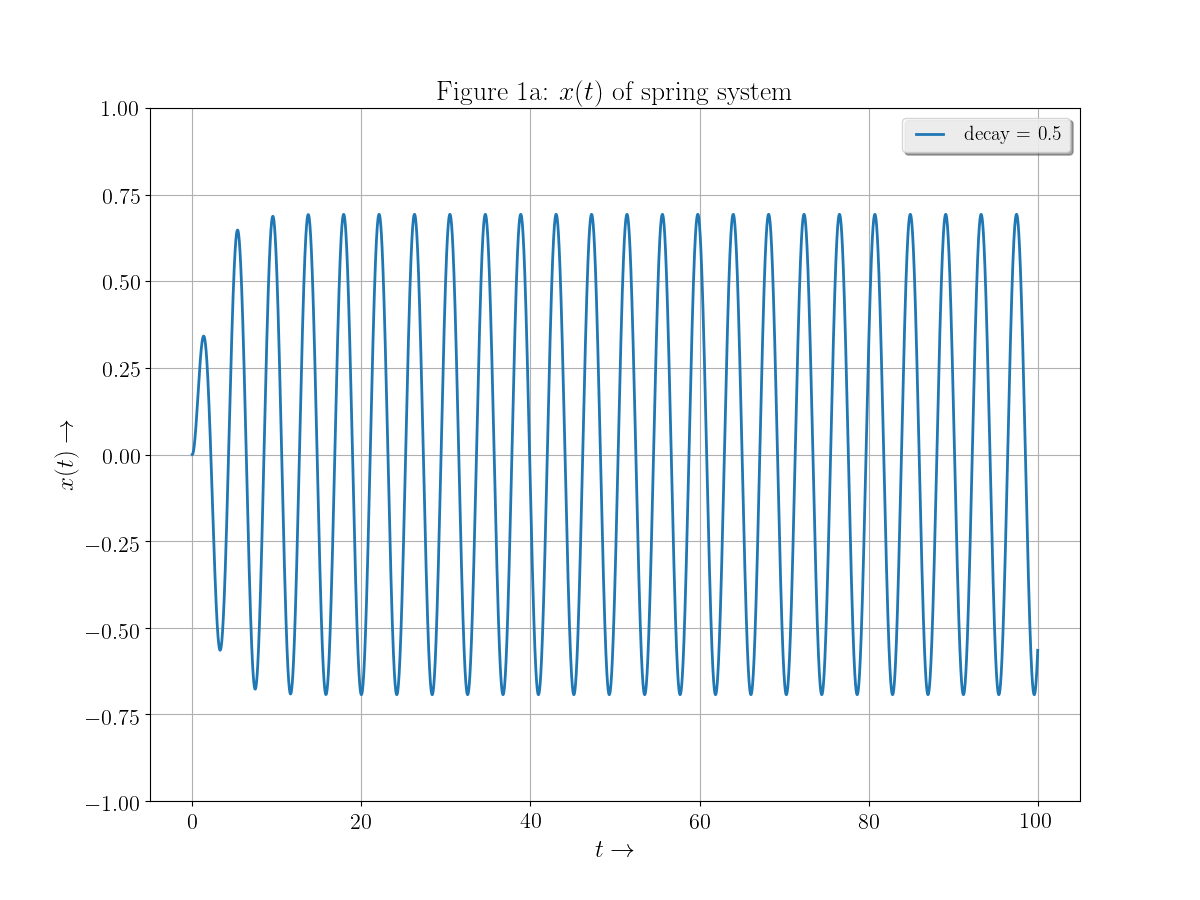
\includegraphics[scale=0.4]{./../Extras/A61a.png}  % Mention the image name within the curly braces. Image should be in the same folder as the tex file. 
    
    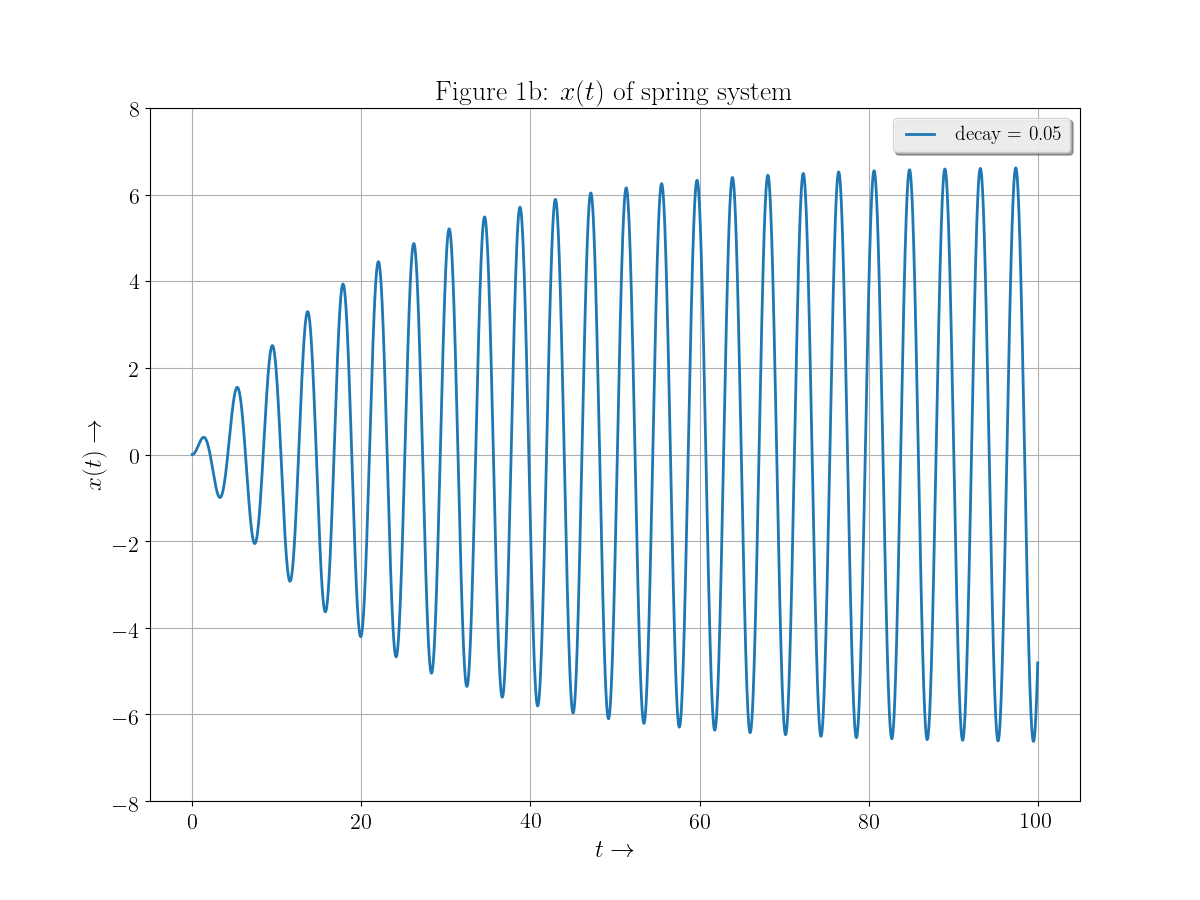
\includegraphics[scale=0.4]{./../Extras/A61b.png}  % Mention the image name within the curly braces. Image should be in the same folder as the tex file. 
    \caption{Plots of displacement of block for two different decays}
  \end{figure}
\newpage
\subsubsection{Results and Discussion :}\label{results-and-discussion}
\begin{itemize}
    \item
      As we observe the plot that for smaller decay of \(e^{-0.05t}\), \(x(t)\) has large amplitude and its growing as
      time increases and oscillates.
    \item
      Whereas the for higher decay value the amplitude of \(x(t)\) is very
      small but since its second order system it oscillates.
    \item
      And If we observe the Figure 1a, amplitude growth stopped and settles
      quicker than for smaller decay value whereas for small decay value
      the \(x(t)\) amplitude settling time is larger because as given below:
    \item
      Our input \(f(t)\) to the system has natural frequency that is
      \(w=w_0\), so its a resonant case,so the solution of differentail
      equation for sinusoidal inputs from observing the plot can be of the
      form \(te^{-dt}\cos (w_0 t)\) so for smaller decay value the graph
      takes more time neutralise the growing effect of \(t\) in the
      solution.
    \item
      So to conclude for small decay , \(x(t)\) has large amplitude and the
      time required for it settle or saturate to a certain maximum amplitude
      is higher compared to large decay case
    \end{itemize}
  \newpage
        \subsection{Question 3:}\label{question-3}
    
    \begin{itemize}
    \item
      In an LTI system. \(f(t)\) is the input, and \(x(t)\) is the output.
    \item
      To Obtain the system transfer function
      \(\frac{\mathcal {X}(s)}{ \mathcal {F}(s)}\)
    \item
      we use \(signal.lsim\) to simulate the problem.
    \item
      Here we try to plot the system response for different values of
      excitation frequecies i.e input frequencies with natural frequency of
      the system as \(w_0 = 1.5 rads^{-1}\)
    \item
      So using a for loop, we sweep the frequency \(w\) of the \(f(t)\) from
      \(1.4\) to \(1.6\) in steps of \(0.05\) keeping the exponent as
      \(e^{−0.05t}\) that is \(d=0.05\) and plot the resulting responses.
    \item
      So with above conditions laplace transform of \(x(t)\) is
    \end{itemize}
    
    \begin{equation}
        \mathcal{X}(s) = \frac{s+0.05}{((s+0.05)^2 + w^2)(s^2 + 2.25)}
    \end{equation}
    
    \begin{itemize}
    
    \item
      So we transfer function of the system is
    \end{itemize}
    
    \begin{equation}
        \mathcal{H}(s) = \frac{s+0.05}{((s+0.05)^2 + w^2)(s^2 + 2.25)}
    \end{equation}
    
    \begin{equation}
        \mathcal{H}(s) = \frac{s+0.05}{((s+0.05)^2 + w^2)(s^2 + 2.25)}
    \end{equation}
    
    \begin{itemize}
    
    \item
      Using this we analyse the results.
    \end{itemize}
    \textit{\textbf{Code:}}
   \begin{lstlisting}
def cosf(t, w, decay):
    return cos(w*t)*exp(-decay*t)

for w in arange(1.4, 1.6, 0.05):
    decay = 0.05
    H, a, b, = laplaceSolver(decay, 1.5)
    t = linspace(0, 200, 20000)
    t, y, svec = sp.lsim(H, cosf(t, w, decay), t)
    plot(t, y, label="$w$ = %g rad/s" % (w))
    legend()
    plot()
xlabel(r"$t \to $")
ylabel(r"$x(t) \to $")
ylim((-80, 80))
title(r"Figure 2: $x(t)$ of spring system with varying frequencies")
grid()
show()
   \end{lstlisting}
   \newpage
   \begin{figure}[!tbh]
    \centering
    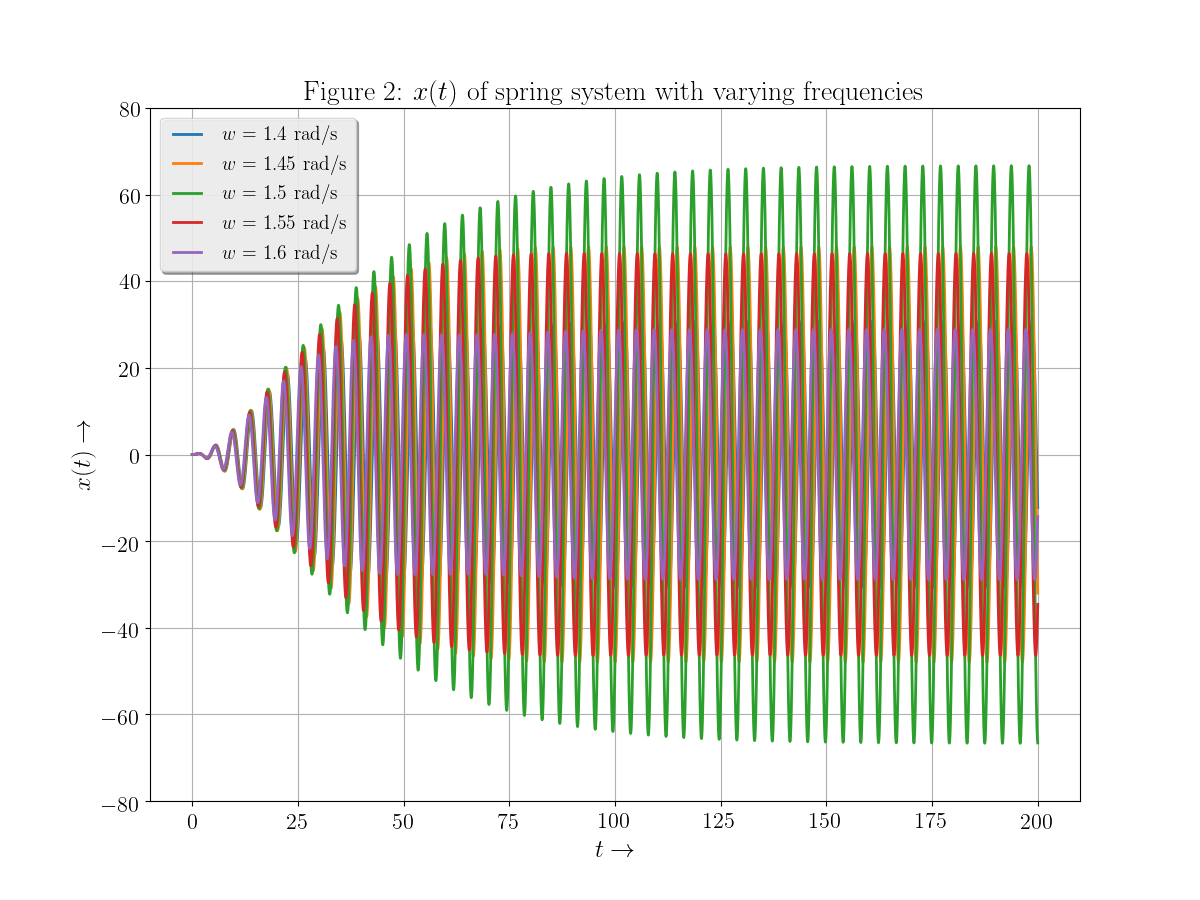
\includegraphics[scale=0.5]{./../Extras/A62.png}  % Mention the image name within the curly braces. Image should be in the same folder as the tex file. 
        \caption{Plots of displacement of block for different frequencies}
  \end{figure}
  \newpage
  \subsubsection{Results and Discussion:}\label{results-and-discussion}
\begin{itemize}
\item
We see that for frequency $\omega = 1.5 rads^{-1}$, the amplitude is the largest since it is the resonance frequency of the system.
\item
  As we observe in Figure 2 that when we force (we are basically exciting
  the spring mass system with \(f(t)\)) the system with \(w \neq w_0\)
  where \(w_0 = 1.5\) and \(w \approx w_0\) i.e around 1.5
  \(rads^{-1}\),since intially the system is at rest,so when f(t) is
  forced upon it,they are in phase,so constructive superposition occurs
  so the amplitude of \(x(t)\) increases in same fashion for \(w\) very
  close to \(w_0\) at starting , after that since the forced and natural
  frequency are not same,it is detuned so amplitude after peak amplitude
  starts falling slightly but at steady state all forced response dies
  out,so basically \(x(t)\) will vary only with natural mode since
  forced response died out eventually.
\item
  Whereas for \(w=w_0\) case resonant occurs,so system and forcing input
  have same frequency so,the forced response adds up to natural response
  basically 'tuned',so the amplitude is very high in steady state.
\end{itemize}
\newpage
    \subsection{Question 4:}\label{question-4}

\begin{itemize}
\item
  To Solve for a coupled spring problem:
\item
  System satisfies the below equation with \(x(0) = 1\) and
  \(\dot x(0) = y(0) = \dot y(0) = 0\).
\end{itemize}

\begin{equation}
\ddot x + (x-y) = 0
\end{equation}

\begin{equation}
\ddot y + 2(y-x)= 0
\end{equation}

\begin{itemize}
\item
  Solve for $x(t)$ and $y(t)$ for $ 0 \leq t \leq 20s$ by taking
  laplace transform of both equations given above and solve for
  \(\mathcal {X}(s)\) and \(\mathcal{Y}(s)\) using substitution method.
\item
  Now from \(\mathcal {X}(s)\) and \(\mathcal{Y}(s)\) find \(x(t)\) and
  \(y(t)\) using \(system.impulse\).
\item
  Plot \(x(t)\) and \(y(t)\) in the same graph and analyse them
\end{itemize}
\textit{\textbf{Code:}}
\begin{lstlisting}
def coupledSysSolver(n_coeff, d_coeff):
    H_n = poly1d(n_coeff)
    H_d = poly1d(d_coeff)

    Hs = sp.lti(H_n, H_d)
    t, h = sp.impulse(Hs, None, linspace(0, 100, 1000))
    return t, h


t1, x = coupledSysSolver([1, 0, 2], [1, 0, 3, 0])
t2, y = coupledSysSolver([2], [1, 0, 3, 0])

plot(t1, x, 'b', label="$x(t)$")
plot(t2, y, 'r', label="$y(t)$")
legend()
title(r"Figure 3: Time evolution of $x(t)$ and $y(t)$ for $0 \leq t 
\leq 100$. of Coupled spring system ")
xlabel(r"$t \to $")
ylabel(r"$x(t),y(t) \to $")
ylim((-0.5, 2))
grid()
show()
\end{lstlisting}
\newpage
\begin{figure}[!tbh]

  \centering
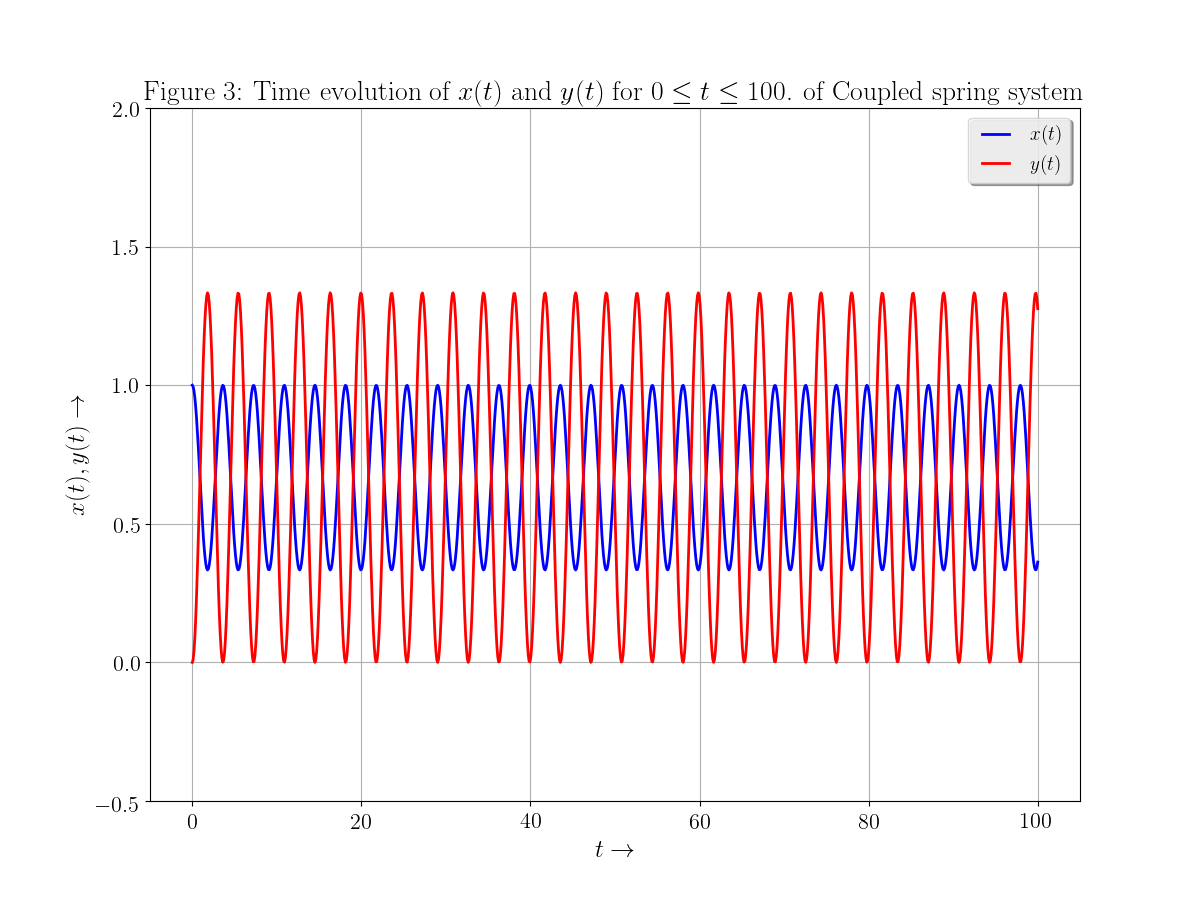
\includegraphics[scale=0.5]{./../Extras/A63.png}  % Mention the image name within the curly braces. Image should be in the same folder as the tex file. 
    \caption{Plots of displacement of two coupled blocks}
\end{figure}
\newpage
\subsubsection{Results and Discussion:}\label{results-and-discussion}

\begin{itemize}

\item
  As we observe figure 4 that, the \(x(t)\) and \(y(t)\) obtained
  satisfies the given initial conditions,and oscillating sinusoidally
  with \(180^{o}\) out of phase
\end{itemize}
\newpage
    \subsection{Question 5:}\label{question-5}

\begin{itemize}
\item
  To Obtain the magnitude and phase response of the Steady State
  Transfer function of the following two-port network
\item
  Transfer function of the RLC network from input to voltage at
  capacitor in general for given Network is
\end{itemize}

\begin{equation}
    \frac{\mathcal{V} _{0}(s)}{\mathcal{V}_{i}(s)} = \mathcal{H}(s) = \frac{1}{s^{2}LC + sRC + 1}
\end{equation}

\begin{itemize}
\item
  For the given values of $ R = 100 \Omega\ , L = 1\mu H,C= 1\mu F$
\item
  We get
\end{itemize}

\begin{equation}
    \mathcal{H}(s) = \frac{1}{s^{2}10^{-12} + s10^{-4} + 1}
\end{equation}

\begin{itemize}

\item
  can be written as
\end{itemize}

\begin{equation}
    \mathcal{H}(s) = \frac{1}{(1 + \frac{s}{10^{8}})(1 + \frac{s}{10^{4}})}
\end{equation}

\begin{itemize}
\item
  So system has poles on left half s plane, that too real poles with $
  s = -10^{4},-10^{8}$ $rads^{-1}$, we will observe the
  effect of poles on magnitude and phase response by analysing plots of
  them
\item
  Magnitude Response is \(|H(s)|\) evaluated at any point on imaginary
  axis so basically \(|H(j\omega)|\)
\item
  Phase response is \(\angle H(j\omega)\)
\item
  Using \(\mathcal{H}(s)\) we calculate magnitude and phase response of
  it using \(Bode()\) and plot them and analyse.
\end{itemize}

\textit{\textbf{Code:}}
\begin{lstlisting}
  
def RLCnetwork(R, C, L):
  Hnum = poly1d([1])
  Hden = poly1d([L*C, R*C, 1])

  Hs = sp.lti(Hnum, Hden)

  w, mag, phi = Hs.bode()
  return w, mag, phi, Hs


R = 100
L = 1e-6
C = 1e-6

w, mag, phi, H = RLCnetwork(R, L, C)

semilogx(w, mag, 'b', label="$Magnitude Response$")
legend()
title(r"Figure 4: Magnitude Response of $H(jw)$ of Series 
RLC network")
xlabel(r"$ \log w \to $")
ylabel(r"$ 20\log|H(jw)|  \to $")
grid()
show()

semilogx(w, phi, 'r', label="$Phase Response$")
legend()
title(r"Figure 5: Phase response of the $H(jw)$ of Series RLC 
network for")
xlabel(r"$ \log w \to $")
ylabel(r"$ \angle H(j\omega)$ $\to $")
grid()
show()
\end{lstlisting}
\newpage
\begin{figure}[!tbh]

  \centering
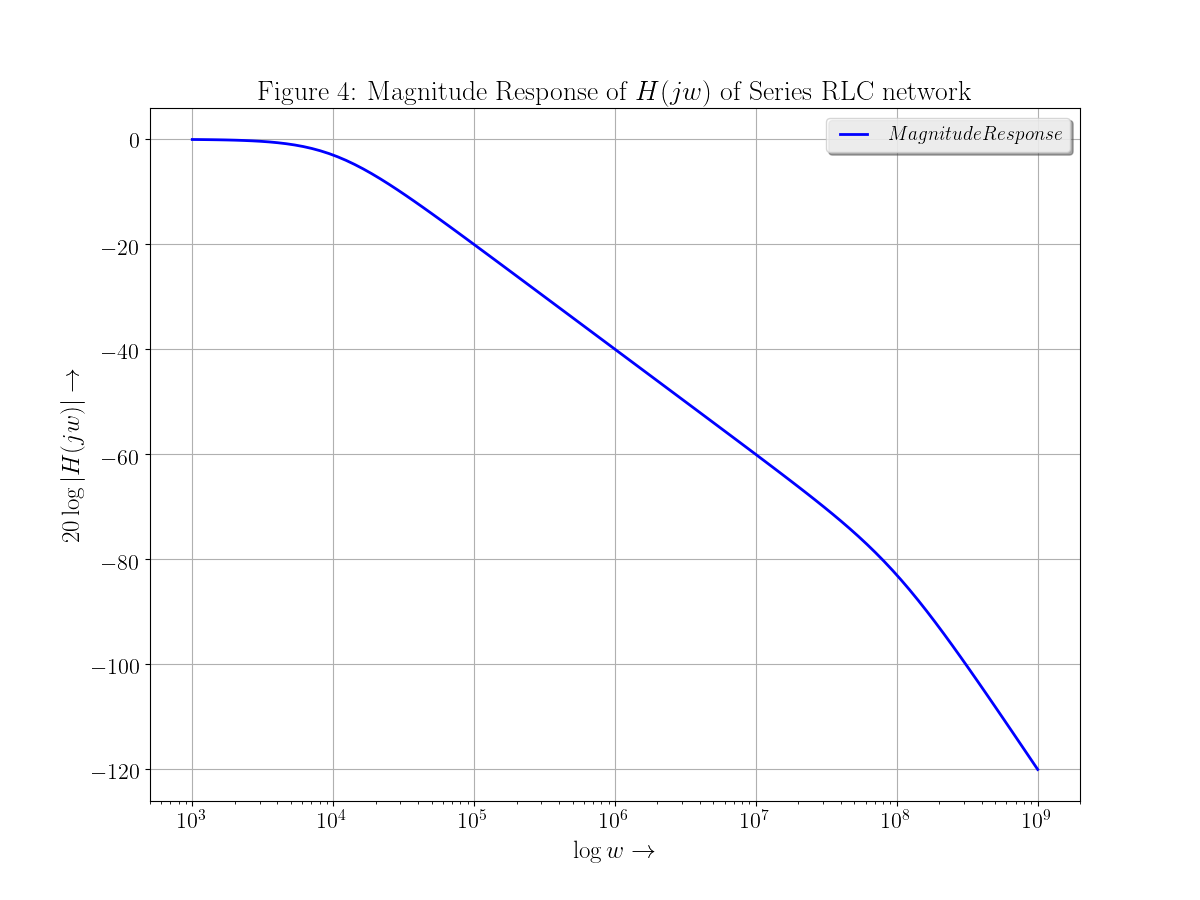
\includegraphics[scale=0.4]{./../Extras/A64.png}  % Mention the image name within the curly braces. Image should be in the same folder as the tex file. 
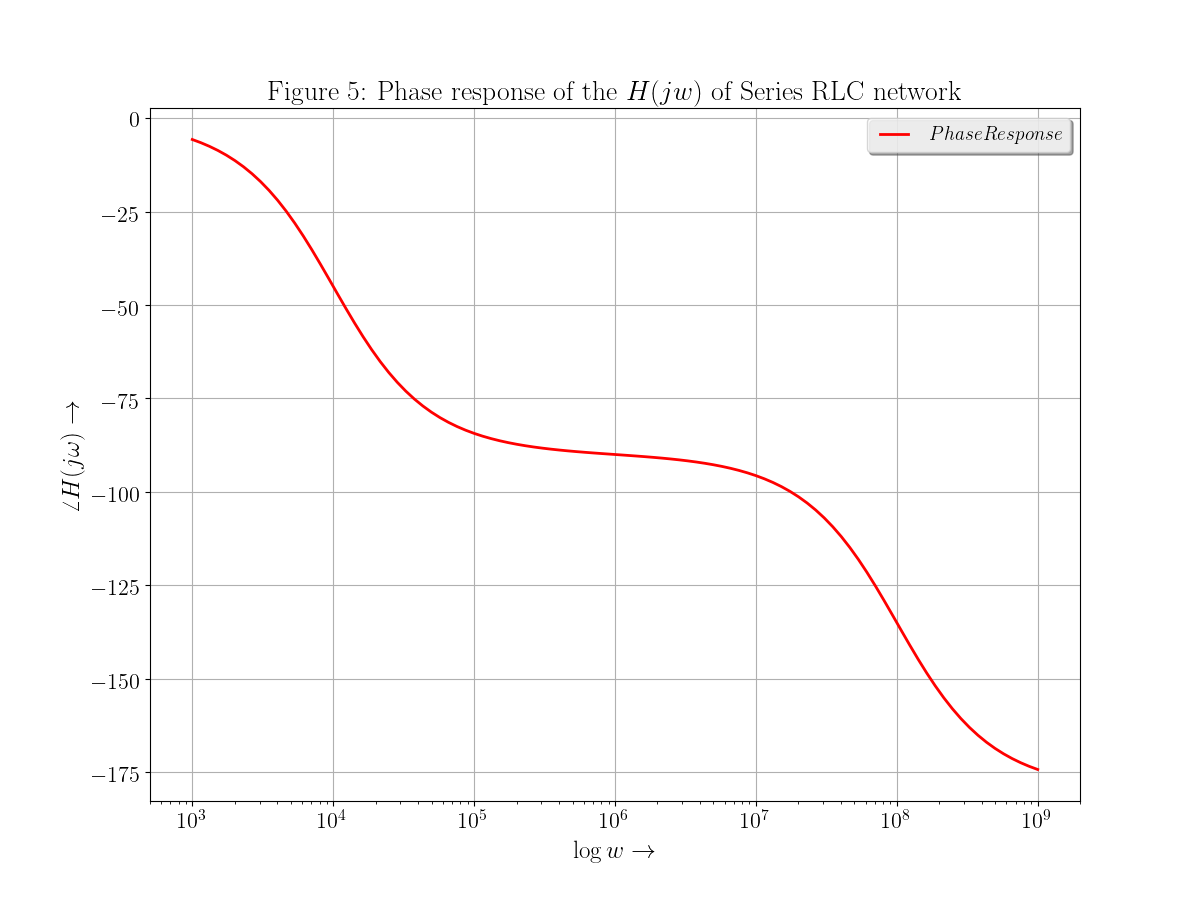
\includegraphics[scale=0.4]{./../Extras/A65.png}  % Mention the image name within the curly braces. Image should be in the same folder as the tex file. 

\caption{Bode Plots of the LCR system}
\end{figure}

\newpage
\subsubsection{Results and Discussion:}\label{results-and-discussion}

\begin{itemize}
\item
  As we observe figure 6 that,\(0 \leq \angle H(j\omega) < 180^{o}\).
\item
  So the system is unconditionally stable since phase does not go to
  \(180^{o}\).
\item
  Since each pole adds \(90^{o}\) to the phase its clear that the system
  is second order because it has two poles hence phase go till
  \(180^{o}\).
\item
  And since all the poles are in left half s plane RLC Network given is
  unconditionally stable for given values.
\end{itemize}
\newpage

    \subsection{Question 6:}\label{question-6}

\begin{itemize}
\item
  Consider the problem in \(Q5\).If the input signal \(v_i(t)\) is given
  by
\end{itemize}

\begin{equation}
 v_i(t) = \cos (10^{3}t) u(t) − \cos (10^{6}t) u(t)
 \end{equation}

\begin{itemize}
\item
  Obtain the output voltage \(v_0(t)\) using the transfer function of
  the system obtained.
\item
  To explain the output signal for $ 0 \textless{} t \textless{} 30
  \mu s $
\item
  And explain the long term response on the \(msec\) timescale
\end{itemize}
\textit{\textbf{Code:}}
\begin{lstlisting}
  
t = linspace(0, 90*pow(10, -3), pow(10, 6))
vi = cos(t*pow(10, 3))-cos(t*pow(10, 6))

t, vo, svec = sp.lsim(H, vi, t)
vo_ideal = cos(1e3*t)

plot(t, vo, 'r', label="Output voltage $v_0(t)$ for large time")
legend()
title(r"Figure 6a: Output voltage $v_0(t)$  of series RLC network
 for given $v_i(t)$ at Steady State")
xlabel(r"$ t \to $")
ylabel(r"$ y(t) \to $")
grid()
show()

plot(t, vo, 'r', label="Output voltage $v_0(t)$ - zoomed in ")
plot(t, vo_ideal, 'g', label="Ideal Low Pass filter Output with
 cutoff at $10^4$")
xlim(0.0505, 0.051)
ylim(0.75, 1.1)
legend()
title(r"Figure 6b: Output voltage $v_0(t)$  Vs Ideal Low pass
 filter Output")
xlabel(r"$ t \to $")
ylabel(r"$ y(t) \to $")
grid()
show()

plot(t, vo, 'r', label="Output voltage $v_0(t)$ : $0<t<30\mu sec$")
legend()
title(r"Figure 7: Output voltage $v_0(t)$ for $0<t<30\mu sec$")
xlim(0, 3e-5)
ylim(-1e-5, 0.3)
xlabel(r"$ t \to $")
ylabel(r"$ v_0(t) \to $")
grid()
show()
\end{lstlisting}
\newpage
\begin{figure}[!tbh]

  \centering
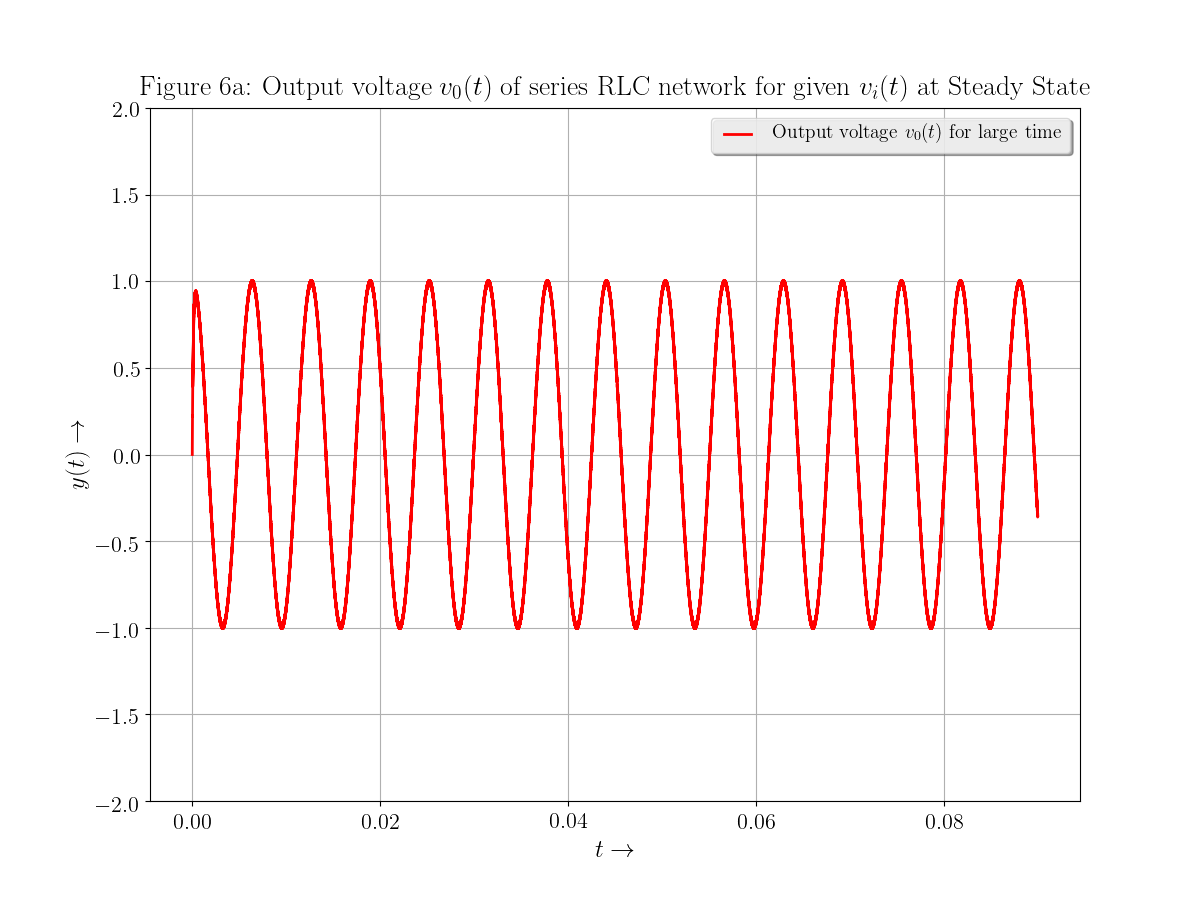
\includegraphics[scale=0.4]{./../Extras/A66a.png}  % Mention the image name within the curly braces. Image should be in the same folder as the tex file. 
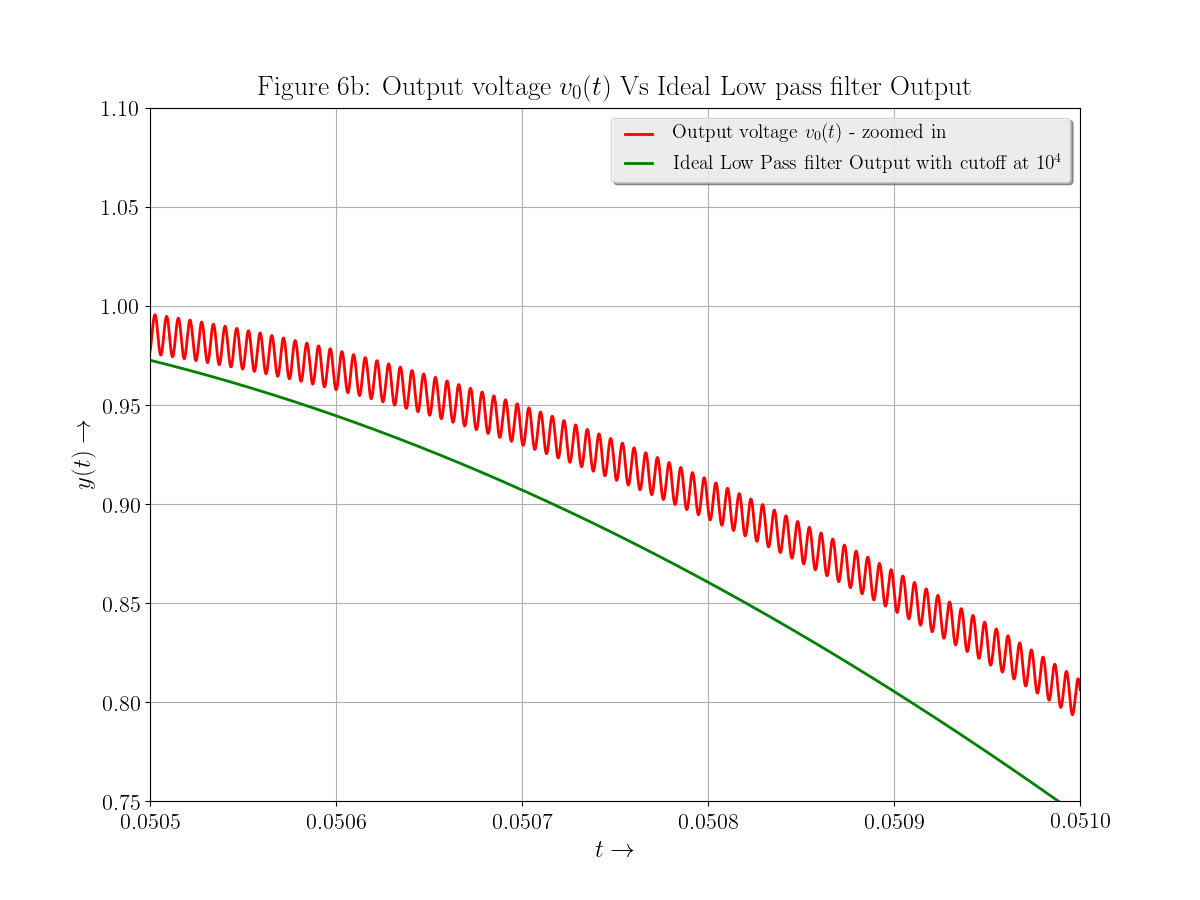
\includegraphics[scale=0.4]{./../Extras/A66b.png}  % Mention the image name within the curly braces. Image should be in the same folder as the tex file. 

\caption{Output of the LCR system(LPF) and comparision with Ideal LPF}
\end{figure}
\newpage
\begin{figure}[!tbh]

  \centering
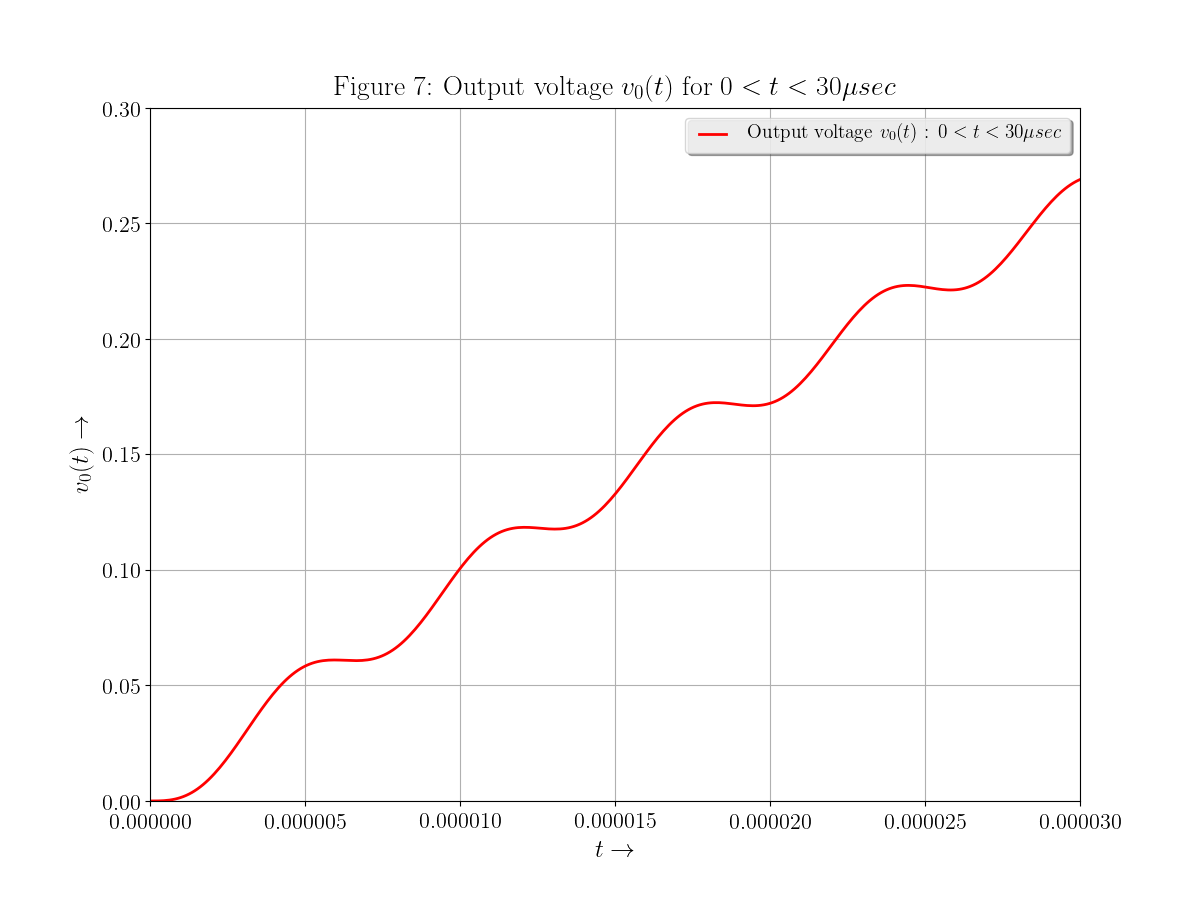
\includegraphics[scale=0.5]{./../Extras/A67.png}  % Mention the image name within the curly braces. Image should be in the same folder as the tex file. 


\caption{Initial plot for time between 0 to 30 $\mu$s}
\end{figure}
\newpage
\subsubsection{Results and Discussion:}\label{results-and-discussion}

\begin{itemize}
\item
  As we observe the plot and the circuit that we know it is a Low pass
  filter with bandwidth \(0< \omega < 10^4\).
\item
  So when the circuit will only pass input with frequencies which are in
  range of bandwidth only. But since its not a ideal low pass filter as
  its gain doesn't drop abruptly at \(10^4\) rather gradual decrease
  which is observed from magnitude response plot.
\item
  So the output \(V_o(t)\) will be mainly of \(\cos(10^{3}t)\) with
  higher frequencies riding over it in long term response i.e Steady
  state solution.
\item
  This behaviour is observed in the plot that,the
  \(v_o(t) \approx \cos(10^{3}t)\) with higher frequencies riding over
  it for large time.
\item
  The curve is very flickery or not smooth because of the high frequency
  components only.
\item
  In the next plot we've zoomed large enough to observe those components.
\end{itemize}
\begin{itemize}
  \item
    The oscillatory behaviour in the graph is because of high frequency
    components riding over the main signal which is \(\cos(10^{3}t)\)
    since gain of the system \(\approx 1\) for lower frequencies than
    \(\omega < 10^4\) and gradually decreases as 20dB/dec which is
    observed from magnitude response plot and for very high frequencies
    40dB/dec.
  \item
    So there will be some higher frequencies but the gain will be very
    less since its low pass filter ,that's why we can see there are very
    small sinusoidal oscillations over the main output signal compared to
    ideal low pass filter output which is \(\cos(10^{3}t)\)
  \end{itemize}
  \begin{itemize}
    \item
      As we observe the plot of Figure 6 , for \(v_0(t)\) from
      \(0<t<30\mu sec\) increases very fast from 0 to 0.3 in just
      \(30\mu s\) because of transients that is we apply sinusoidal step
      input to the system i.e the input is zero for \(t<0\), so when
      abruptly the input becomes non zero for \(t \geq 0\), the system
      output jumps or raises suddenly from 0 to non-zero values in less
      time.
    \item
      That's why we observe a sharp rise in output at the start.
    \item
      And the oscillatory behaviour in the graph is because of high
      frequency components riding over the main signal which is
      \(\cos(10^{3}t)\) since gain of the system \(\approx 1\) for lower
      frequencies than \(\omega < 10^4\).
    \end{itemize}
    \section{Conclusion:}\label{conclusion}

    \begin{itemize}
    \item
      So to conclude we analysed a way to find the solution of continuous
      time LTI systems using laplace transform with help of Python signals
      toolbox and got familiarised with solving of differential equations by
      taking laplace transform instead of doing arduous time domain
      analysis.
    \end{itemize}
    
      
\end{document}